\documentclass[sigconf,nonacm]{acmart}
\usepackage{algorithm}
\usepackage{algpseudocode}
%%
%% \BibTeX command to typeset BibTeX logo in the docs
\AtBeginDocument{%
  \providecommand\BibTeX{{%
    Bib\TeX}}}


\begin{document}

\title{Reimagining Transit Networks: A Data-Driven, Algorithmic Approach for the Washington DC Region}

\author{Spencer Jenkins}

\renewcommand{\shortauthors}{S. Jenkins}

\begin{abstract}
This paper presents a computational framework for the design and economic evaluation of reimagined rapid transit networks for the Washington, DC metropolitan area. Motivated by the historical limitations of the existing WMATA system, this study leverages geospatial analysis, multi-hop graph neighborhood aggregation, and multiple network generation approaches---including heuristic random walks, an iterative improvement method, a MAX-MIN Ant Colony System~\cite{stutzle2000mmas,nikolic2013aco}, and a genetic algorithm---to generate and evaluate alternative transit networks. Origin-destination employment data from the LEHD LODES dataset~\cite{lodes2023} augments population-based demand signals, while OpenStreetMap right-of-way classification~\cite{boeing2017osmnx} enables per-segment construction cost estimation calibrated to FTA benchmarks~\cite{fta2023ntd,flyvbjerg2003overruns}. A doubly-constrained gravity model~\cite{wilson1971gravity} calibrated to a WMATA-scale ridership target provides station-level boarding estimates disaggregated by time of day. The resulting networks outperform the real-world WMATA network on key coverage metrics: point coverage (up to 16.5\%), neighborhood coverage (up to 7.0\%), and average distance to the nearest station (as low as 0.99\,km in DC). These results demonstrate the potential of data-driven, algorithmically optimized approaches to improve urban mobility and equity in transit planning.
\end{abstract}

\maketitle



\section{Introduction}

Public transportation is a vital component of urban infrastructure, contributing to economic productivity~\cite{lit:us_transit_policy}, social equity~\cite{lit:equity}, and environmental sustainability~\cite{lit:us_transit_policy} in metropolitan areas. Washington, DC, and its surrounding areas in Maryland and Virginia, are served by a six-line heavy rail system spanning about 208 kilometers and connecting 98 stations, operated by the Washington Metropolitan Area Transit Authority (WMATA)~\cite{lit:wmata_wikipedia}. Recent annual ridership is on the order of hundreds of millions of trips~\cite{lit:wmata_wikipedia}. Figure~\ref{fig:wmata} provides a reference for the existing transit network, which is compared to the generated networks throughout this study. 
% --- Figure: Real-World Transit Network ---
\begin{figure}[ht]
    \centering
    \includegraphics[width=0.23\textwidth]{./img/wmata.png}
    \caption{Map of the real-world WMATA transit network in the Washington, DC region.}
    \label{fig:wmata}
    \Description{A map showing the layout of the WMATA rapid transit network in Washington, DC, with colored lines representing different rail routes and station locations.}
\end{figure}

A primary goal in designing public transit networks in the U.S. is to reduce car dependency~\cite{lit:us_transit_policy}. However, the Washington Metro has struggled to achieve this, with only about 14\% of commuters in the region using transit~\cite{lit:commute_stats}. Comparable metropolitan areas such as Toronto report higher transit commute shares, while many European and Latin American cities also have significantly higher shares~\cite{lit:toronto}. These statistics are typically limited to work commutes, as data for other trip types is less available~\cite{lit:commute_stats}.

The limited success of the Washington Metro in attracting ridership is largely attributable to the priorities at the time of its planning~\cite{lit:wmata_history}. Unlike older East Coast cities with legacy rail systems, the Metro was conceived in the 1950s, an era of expanding car infrastructure and urban expressways. The Metro was designed as a compromise, connecting car commuters to the city center, with expansions primarily serving suburban areas~\cite{lit:wmata_history}. As a result, the network remains largely radial and focused on suburban commuters.

This design philosophy limits practical use. The largely radial structure makes suburb-to-suburb and circumferential travel difficult, often requiring trips to route through the core and transfer. High-density neighborhoods such as Georgetown and marginalized areas like Anacostia have been historically underserved due to political, financial, and social factors~\cite{lit:equity}. Despite significant investment, the Metro has not achieved a substantial reduction in vehicle miles traveled (VMT) or car dependency~\cite{lit:env}. The static nature of the network has also hindered adaptation to shifting population centers and job clusters.

The persistent gaps in the current network's ability to connect high-density and underserved regions further motivate a new approach. For example, the lack of direct connections between major suburban job centers or marginalized neighborhoods limits economic opportunity and social inclusion~\cite{lit:equity}. Existing evaluation frameworks may overlook these gaps, focusing on aggregate metrics that mask disparities in access and service quality.

To address these challenges, this study asks: \textit{Can data-driven, algorithmically generated rapid transit networks for the Washington, DC region outperform the existing WMATA system on coverage, equity, and access metrics?} This paper makes the following contributions: (1) a demand-weighted spatial graph construction pipeline combining census, employment, and point-of-interest data; (2) four distinct transit network generation algorithms---constrained random walks, iterative improvement, MAX-MIN Ant Colony Optimization, and a genetic algorithm---applied to the same spatial search space; (3) per-segment construction cost estimates via OpenStreetMap right-of-way classification; (4) station-level ridership modeled using a doubly-constrained gravity model; and (5) a multi-metric evaluation against the real-world WMATA network on coverage, equity, and transfer burden.


% --- Table: Counties and FIPS codes ---

% Table 1: Counties and County-Equivalents Considered

\begin{table*}[h]
\caption{Counties and County-Equivalents in the Study Area}
\label{tab:counties}
\resizebox{\textwidth}{!}{
\begin{tabular}{lccc}
\toprule
County/Equivalent & 2020 Population & Density (per km$^2$) & FIPS Code \\
\midrule
Prince George's & 967,201 & 687 & 24033 \\
Montgomery & 1,062,061 & 849 & 24031 \\
District of Columbia & 689,545 & 4,457 & 11001 \\
Arlington County & 238,643 & 3,672 & 51013 \\
Alexandria City & 159,467 & 4,293 & 51510 \\
Falls Church City & 14,658 & 2,651 & 51610 \\
Fairfax County & 1,150,309 & 1,184 & 51059 \\
Fairfax City & 24,146 & 1,563 & 51600 \\
Loudoun County & 420,959 & 334 & 51107 \\
\bottomrule
\end{tabular}
}
\end{table*}

% Add citation for census data
\noindent\textit{Source: U.S. Census Bureau, QuickFacts, 2020 Census Redistricting Data (Public Law 94-171) Summary File~\cite{lit:census}.} 

% --- Table: Data Sources ---

\begin{table*}[h]
\caption{Key Data Sources Used in the Study}
\label{tab:datasources}
\resizebox{\textwidth}{!}{
\begin{tabular}{ll}
\toprule
Source & Description \\
\midrule
US Census Bureau TIGER/Line~\cite{lit:tiger2023} & Census block shapefiles \\
American Community Survey~\cite{lit:acs2022} & Socioeconomic equity features \\
Open Data DC/MD/VA & Points of interest, land use \\
Arlington County & Neighborhood boundaries \\
State of Maryland & Neighborhood boundaries \\
District of Columbia & Neighborhood centroids \\
WMATA & Existing transit network \\
US Census Bureau LEHD~\cite{lodes2023} & Block-level employment OD flows (LODES8) \\
OpenStreetMap via OSMnx~\cite{boeing2017osmnx} & Road and rail geometry for ROW classification \\
\bottomrule
\end{tabular}
}
\end{table*}

\section{Literature Review}

The design and optimization of transit networks intersects transportation engineering, computer science, social science, and operations research. This section summarizes a review of relevant literature on geospatial data structures, network generation algorithms, and optimization approaches for transit planning.

Efficient representation and querying of spatial data is foundational for transit network design. Classic work by Libera~\cite{bib:libera1986btrees} introduced B-tree structures for geographic information systems, enabling rapid spatial queries and hierarchical decomposition of map regions. Samet et al.~\cite{bib:samet1984quadtrees} are well known for introducing quadtree structures for spatial data, supporting hierarchical decomposition in GIS applications. These data structures inspire the recursive spatial partitioning and point selection methods used to identify high-need transit locations. Toman and Olszewska~\cite{toman2014algorithm} further demonstrate how geographic data can be transformed into network graphs, a process analogous to the use of census and point-of-interest data to construct candidate station and edge sets.

A variety of algorithmic approaches have been proposed for generating and optimizing transit networks. Bast et al.~\cite{bast2016route} provide a comprehensive overview of route planning algorithms in transportation networks, including shortest-path, greedy, and metaheuristic methods. Greedy algorithms, as surveyed by Davis and Impagliazzo~\cite{davis2007greedy}, offer computational efficiency for a range of graph problems, though they may yield suboptimal solutions for complex network design tasks. Genetic algorithms (GAs) have been shown to be effective for transit route planning, as demonstrated by Chien et al.~\cite{chien2001genetic} and Dib et al.~\cite{bib:dib2017ga}, who apply GAs to optimize bus and public transit networks under multiple criteria. This study adapts these approaches to rapid transit and also introduces a MAX-MIN Ant System~\cite{stutzle2000mmas} formulation for the Transit Network Design Problem, following Nikolić and Teodorović~\cite{nikolic2013aco}.

Graph neural network approaches have recently been applied to transportation demand modeling. Hamilton et al.~\cite{hamilton2017graphsage} introduce GraphSAGE, an inductive representation learning framework that propagates neighborhood features through mean aggregation. Veličković et al.~\cite{velickovic2018gat} extend this with attention-weighted aggregation (Graph Attention Networks), enabling nodes to selectively weight neighbors by demand-signal relevance. This study applies a numpy-only multi-hop neighborhood aggregation scheme following the GraphSAGE mean-aggregator formulation to re-score graph nodes beyond KDE density; no weight matrices are trained, so the aggregation propagates existing demand signals rather than learning new representations. Employment origin-destination data from the U.S. Census LEHD LODES program~\cite{lodes2023} is used to build commute-pattern-aware demand surfaces that supplement the population-based signal.

Construction cost estimation draws on FTA National Transit Database benchmarks~\cite{fta2023ntd} and Halcrow Fox per-km multipliers~\cite{halcrow2000cost}, with a contingency factor motivated by Flyvbjerg et al.'s~\cite{flyvbjerg2003overruns} meta-analysis of 258 infrastructure projects, which documents a systematic 44.7\% average rail overrun. Right-of-way classification uses OSMnx~\cite{boeing2017osmnx}, following a simplified map-matching strategy in the spirit of Newson and Krumm~\cite{newson2009mapmatching}. Ridership estimation uses Wilson's~\cite{wilson1971gravity} doubly-constrained gravity model, whose calibration is informed by observed ridership patterns in prior gravity-model studies such as Zhao et al.~\cite{zhao2022ridership}.

Recent work has emphasized the importance of equity and real-world constraints in transit planning. Camporeale et al.~\cite{camporeale2016equity} discuss the quantification of horizontal and vertical equity in route planning, motivating the inclusion of coverage metrics for both high-density and underserved areas. Extensions to other modes, such as smart transit and high-speed rail, are explored by P\'erivier et al.~\cite{perivier2021realtime} and Roy and Maji~\cite{roy2023hsr}, whose methodologies for station location optimization and real-time routing offer inspiration for future work.

\section{Network Design}

In this section, the network design process is detailed, including data collection, transformation, metric construction, network generation constraints, and the definition of the transit network search space. The network is built within this search space according to the scoring metrics and constraints, followed by post-processing.

\subsection{Data Sources and Transformation}
The first step is to define the study area. Table~\ref{tab:counties} lists the counties and county-equivalents included, along with their 2020 population, density, and FIPS code~\cite{lit:census}. Figure~\ref{fig:area_considered} shows a map of the included regions.
% --- Figure: Area Considered ---
\begin{figure}[ht]
    \centering
    \includegraphics[width=0.3\textwidth]{./img/area_considered.png}
    \caption{Counties and districts considered as part of the Washington, DC metropolitan area.}
    \label{fig:area_considered}
    \Description{A map highlighting the counties and districts included in the Washington, DC metropolitan area for the study.}
\end{figure}

Data for the Washington Metropolitan Area is available from Open Data DC, Open Data MD, and the Virginia Open Data Portal~\cite{lit:opendata}. Census block population data is obtained from the US Census Bureau TIGER/Line tabblock20 shapefiles~\cite{lit:tiger2023}. Transit potential for each block is derived from population density and transformed to form a point-likelihood surface:
\[
  \mathrm{potential}(b) = \ln\!\left(1 + \frac{\mathrm{POP20}(b)}{\mathrm{ALAND20}(b) + \mathrm{AWATER20}(b)} \times 10^3\right)
\]
where $\mathrm{POP20}(b)$ is the 2020 population of block $b$, and $\mathrm{ALAND20}(b) + \mathrm{AWATER20}(b)$ is the total area in m$^2$. The $\log(1+\cdot)$ transform compresses the heavy right tail of the density distribution. Figure~\ref{fig:city_map} shows the census block boundaries used for population and density analysis.

% --- Figure: Census Block Map ---
\begin{figure}[ht]
    \centering
    \includegraphics[width=0.3\textwidth]{./img/city_map.png}
    \caption{Census block map for the Washington, DC area.}
    \label{fig:city_map}
    \Description{A map showing the boundaries of census blocks in the Washington, DC area, used for population and density analysis.}
\end{figure}

The census block data is transformed by taking $\log(1 + \mathrm{density})$. A recursive spatial tree algorithm identifies the highest-need locations for transit, using a depth of 8, and detailed in Figure \ref{fig:get_points_pseudocode}. The resulting points represent locations with the highest need for transit based on population. Figure~\ref{fig:point_likelihood} visualizes the transformed census block data used to identify high-need locations for transit.

\begin{figure}[h]
\centering
\begin{minipage}{1\linewidth}
\begin{algorithmic}
\Function{GetPoints}{DataFrame $D$, Box $E$, Integer $L$}
    \State Initialize list $IDs \gets [\ ]$
    \If{$L \leq 0$ or number of rows in $D < 2$}
        \State \Return $IDs$
    \EndIf
    \State Sort $D$ by \texttt{point\_likelihood} descending
    \State $P \gets$ second row in sorted $D$
    \State Append $P.\texttt{SID}$ to $IDs$
    \State Define sub-boxes using $P$:
    \State \hspace{1em} $E_{BL} \gets$ bottom-left quadrant of $E$ below and left of $P$
    \State \hspace{1em} $E_{BR} \gets$ bottom-right quadrant of $E$ below and right of $P$
    \State \hspace{1em} $E_{TL} \gets$ top-left quadrant of $E$ above and left of $P$
    \State \hspace{1em} $E_{TR} \gets$ top-right quadrant of $E$ above and right of $P$
    \State Query $D$ for points in each quadrant:
    \State \hspace{1em} $D_{BL} \gets D$ in $E_{BL}$
    \State \hspace{1em} $D_{BR} \gets D$ in $E_{BR}$
    \State \hspace{1em} $D_{TL} \gets D$ in $E_{TL}$
    \State \hspace{1em} $D_{TR} \gets D$ in $E_{TR}$
    \State Recursively collect points:
    \State \hspace{1em} $IDs \gets IDs +$
    \State \hspace{2em} \Call{GetPoints}{$D_{BL}, E_{BL}, L - 1$} $+$
    \State \hspace{2em} \Call{GetPoints}{$D_{BR}, E_{BR}, L - 1$} $+$
    \State \hspace{2em} \Call{GetPoints}{$D_{TL}, E_{TL}, L - 1$} $+$
    \State \hspace{2em} \Call{GetPoints}{$D_{TR}, E_{TR}, L - 1$}
    \State \Return $IDs$
\EndFunction
\end{algorithmic}
\caption{Recursive spatial decomposition and top-point selection in a 2-D geographic space.}
\label{fig:get_points_pseudocode}
\end{minipage}
\Description{Points algorithm.}
\end{figure}

% --- Figure: Transformed Census Block Data ---
\begin{figure}[ht]
    \centering
    \includegraphics[width=0.3\textwidth]{./img/point_likelihood.png}
    \caption{Transformed census block data representing input to the recursive spatial algorithm.}
    \label{fig:point_likelihood}
    \Description{A heatmap or point map visualizing transformed census block data, highlighting locations with high need for transit.}
\end{figure}

This data is augmented with points for important destinations, as shown in Table~\ref{tab:datasources}. The selection reflects the availability of data from each source. The study also includes all bus and rail stops in the counties listed, to approximate areas of high transit importance. Specifically, the following transit datasets are aggregated: WMATA Metro stations, WMATA bus stops, DC Streetcar stops, MARC Train stations, Purple Line stations, Virginia Railway Express (VRE) stations, Montgomery County Ride On stops, Maryland MTA bus stops, Prince George's County transit stops, and Virginia bus stops within the study area. These stops serve a dual function: they are included as candidate graph nodes, seeding the spatial search space with locations already recognized as transit-important, and they contribute the existing-transit-access component ($\hat{a}$, inverse distance to nearest stop) of the multi-factor demand surface.

A Gaussian kernel density estimate (KDE) with 1,000\,m bandwidth is fit to the selected candidate points~\cite{bib:silverman1986density}. Figure~\ref{fig:kde_heatmap} displays the KDE heatmap used to model spatial demand for transit. Each graph node $v$ is then scored by the mean KDE density over its own location and 16 uniformly-spaced points on a circle of radius $r = 1{,}000$\,m:
\[
  \mathrm{score}_{\mathrm{KDE}}(v) = \frac{10^{10}}{17}\sum_{k=0}^{16}
    \exp\!\Bigl(\hat{f}\bigl(\mathbf{p}_v + r\,\mathbf{e}_k\bigr)\Bigr)
\]
where $\hat{f}(\cdot)$ is the log-KDE, $\mathbf{e}_0 = \mathbf{0}$, and $\mathbf{e}_k = \bigl(\cos\tfrac{2\pi(k-1)}{16},\,\sin\tfrac{2\pi(k-1)}{16}\bigr)$ for $k \geq 1$. The $10^{10}$ factor is a numerical scaling constant. This radial sampling captures the local demand neighbourhood rather than just the point value, so a node at the edge of a dense area scores higher than one at its isolated center.

To incorporate non-population demand and equity considerations, I also build a multi-factor demand surface over census blocks using population density, point-of-interest (POI) proximity, existing transit access, and tract-level American Community Survey (ACS) variables~\cite{lit:acs2022}. The demand score is defined as a weighted, min-max normalized combination:
\[
    D = w_{pop}\hat{p} + w_{poi}\hat{d} + w_{transit}\hat{a} + w_{eq}\hat{e}
\]
where $\hat{p}$ is population density, $\hat{d}$ is POI density within a 1 km radius, $\hat{a}$ is inverse distance to the nearest existing transit stop, and $\hat{e}$ is an equity signal constructed from ACS median income, poverty rate, disability rate, and zero-vehicle household share. These block-level demand features are used in extended evaluation and sensitivity checks.

\begin{table}[h]
\caption{Demand Feature Weights Used for Multi-Factor Scoring}
\label{tab:demandweights}
\begin{tabular}{lc}
\toprule
\textbf{Component} & \textbf{Weight} \\
\midrule
Population density ($w_{pop}$) & 1.00 \\
POI density ($w_{poi}$) & 0.40 \\
Transit access ($w_{transit}$) & 0.25 \\
ACS equity signal ($w_{eq}$) & 0.35 \\
\bottomrule
\end{tabular}
\end{table}

Node importance is further refined using a two-layer multi-hop neighborhood aggregation scheme implemented in pure NumPy, following the GraphSAGE mean aggregator formulation~\cite{hamilton2017graphsage}. Unlike a trained GNN, no weight matrices are learned; the aggregation applies fixed mean pooling to propagate existing demand signals through graph topology. Each node is featurized by its geographic coordinates, log-KDE density, degree, clustering coefficient, and approximate betweenness centrality. Two rounds of mean aggregation propagate these signals according to:
\[
  H_v^{(l)} = \mathrm{ReLU}\!\left(H_v^{(l-1)} + \frac{1}{|N(v)|}\sum_{u \in N(v)} H_u^{(l-1)}\right), \quad l = 1, 2
\]
so a node surrounded by high-demand neighbors scores higher than an isolated node with the same local KDE value. The final per-node score combines the L2 norm of the two-layer embedding with the raw KDE density, both min-max-normalized to $[0, 1]$:
\[
  \mathrm{score}(v) = \widehat{\bigl\|H_v^{(2)}\bigr\|_2} + \hat{\rho}_v
\]
where $\widehat{\cdot}$ denotes min-max normalization and $\hat{\rho}_v = \exp\!\bigl(\hat{f}(\mathbf{p}_v)\bigr)$ is the KDE density at node $v$. An optional Graph Attention Network variant~\cite{velickovic2018gat} with trained attention weights is available when PyTorch Geometric is installed. These graph-aware node scores replace the pure-KDE scores used in all subsequent route generation stages.

Employment origin-destination data from the LEHD LODES8 program~\cite{lodes2023} is downloaded for DC, MD, and VA (2021 OD main files). Block-level OD pairs are aggregated to census tract level using an 11-character GEOID prefix, and the top 5,000 OD pairs by job count are retained to keep the demand surface computationally tractable. For each retained pair, the workplace census tract centroid is used as the demand point and weighted by its normalized job-flow volume. The resulting data provides a set of demand-weighted points that feed directly into the ACO fitness function (see Section~\ref{sec:network_aco}). This commute-pattern-aware signal ensures that major employment clusters---the Pentagon, NIH, Tyson's Corner---receive appropriate demand weighting independent of residential population density.

% --- Figure: KDE Heatmap ---
\begin{figure}[ht]
    \centering
    \includegraphics[width=0.3\textwidth]{./img/kde.png}
    \caption{Kernel density estimation (KDE) heatmap of population and transit demand in the Washington, DC region.}
    \label{fig:kde_heatmap}
    \Description{A heatmap showing the kernel density estimation of population and transit demand across the Washington, DC region.}
\end{figure}



A mesh of candidate transit points is generated to balance spatial coverage with computational tractability. Population-based points (census block centroids) are combined with non-population points and deduplicated. The Gabriel graph~\cite{gabriel1969} constructed using \texttt{libpysal.weights.Gabriel} connects mutually closest points, resulting in a proximity network suitable for transit planning. The Gabriel graph is converted to a \texttt{networkx} graph for further manipulation, including assignment of edge weights based on Euclidean distance. This mesh serves as the substrate for both random walk and genetic algorithm-based network generation.

A Gabriel graph is constructed using the points. The graph is contracted by condensing Louvain communities~\cite{blondel2008louvain} by a user-defined threshold, forming the overall search space for the network. The network is constructed from the nodes and edges of this graph.

With the data fully preprocessed, one of four network construction algorithms (naive, iterative, genetic, or ACO) is used to determine which line segments from the contracted Gabriel graph become part of the transit network. Across all four methods, fixed no-go zones are enforced around the White House and U.S. Capitol (900\,m buffers) so generated routes avoid protected federal core areas. Figure~\ref{fig:contracted_gabriel} shows the contracted Gabriel graph used as the basis for candidate network construction.

% --- Figure: Contracted Gabriel Graph ---
\begin{figure}[ht]
    \centering
    \includegraphics[width=0.3\textwidth]{./img/graph.png}
    \caption{Contracted Gabriel graph representing the search space for network generation.}
    \label{fig:contracted_gabriel}
    \Description{A network graph visualization showing the contracted Gabriel graph used as the search space for transit network generation.}
\end{figure}


\subsection{Network Creation: Naive (Random Walk) Algorithm}

The naive method involves constrained walks through the graph. The walk procedure is detailed in Figure \ref{fig:perform_walks_pseudocode}. Each walk starts from a random, previously unexplored node and follows the available edge leading to the greatest score. For each subsequent step, the walk chooses an available edge according to a weighted distribution: 75\% probability for the straightest angle, 25\% for the highest KDE score. Only edges forming at least a 130-degree angle from the previous edge can be chosen, and if the overall trajectory deviates by more than 80 degrees, the walk must proceed down edges that bring the angle back. If the walk reaches a node with no options, it terminates and attempts to continue from the original endpoint in the opposite direction. The walk is only kept if it is within a specified length range (45--100 km).

Edges are available if they are unexplored or have been explored up to three times. This reflects the interlined nature of the WMATA Metro, where several lines share alignments.

\begin{figure}[h]
\centering
\begin{minipage}{1\linewidth}
\begin{algorithmic}
\Function{PerformWalks}{Graph $G$, Positions $P$, Parameters}
    \State Initialize $walks$, $threeCount$, $traversedEdges$, $completeTraversedEdges$
    \For{$i \gets 1$ to $numWalks$}
        \State Choose random unvisited $start$ node
        \State Initialize $walk \gets [start]$, $reverseWalk \gets [start]$
        \State Initialize $distance \gets 0$, $totalTurn \gets 0$, $sign \gets 0$
        \While{$distance < maxDistance$}
            \State $(next, deviation, angle) \gets$ \Call{GetNextEdge}{$G, walk[-1], prev, visited, sign$} \State This function chooses an edge based on angle and score
            \If{no valid $next$ and already reversed}
                \State \textbf{break}
            \ElsIf{no valid $next$}
                \State Reverse walk direction, adjust $sign$
                \State \textbf{continue}
            \EndIf
            \State Extend walk with $next$, update $distance$ and $totalTurn$
            \State Update $sign$ based on $totalTurn$
        \EndWhile
        \If{$distance > minDistance$}
            \State Append $walk$ to $walks$
            \State Track traversed edges and update counts
            \State Add frequently used edges to $traversedEdges$
        \Else
            \State Retry with new start node (with timeout)
        \EndIf
    \EndFor
    \State \Return $walks$, $traversedEdges$, $completeTraversedEdges$
\EndFunction
\end{algorithmic}
\caption{Pseudocode for directionally-constrained random walks to generate a transit network over a spatial graph.}
\label{fig:perform_walks_pseudocode}
\end{minipage}
\Description{Walk algorithm}
\end{figure}

\subsection{Network Creation: Iterative Improvement Algorithm}

The iterative improvement method initializes a set of random walks. Walks are scored by the sum of KDE scores for all nodes, indicating transit utility. The lowest-scoring walk is replaced with a newly generated walk, and this process is repeated up to 20 times.

\begin{figure}[h]
\centering
\begin{minipage}{1\linewidth}
\begin{algorithmic}
\Function{IterativeImprovement}{Graph $G$, Positions $P$, KDE $\hat{f}$, $N_{iter}$}
    \State $(W, T, T') \gets$ \Call{PerformWalks}{$G$, $P$, $N_w$ walks, $T{=}\emptyset$, $T'{=}[]$}
    \For{$i \gets 1$ to $N_{iter}$}
        \State $j \gets \arg\min_{k} S_{\mathrm{KDE}}(W_k)$  \Comment{Index of lowest-scoring line}
        \State $(W', T, T') \gets$ \Call{PerformWalks}{$G$, $P$, $N_w{=}1$, $T$, $T'$}
        \State $W_j \gets W'[0]$  \Comment{Replace lowest-scoring line}
    \EndFor
    \State \Return $W$
\EndFunction
\end{algorithmic}
\caption{Pseudocode for the iterative improvement network generation algorithm.}
\label{fig:iterative_pseudocode}
\end{minipage}
\Description{Iterative improvement algorithm pseudocode}
\end{figure}

\subsection{Network Creation: Ant Colony Optimisation}
\label{sec:network_aco}

The ACO stage implements a MAX-MIN Ant System (MMAS)~\cite{stutzle2000mmas} adapted to the Transit Network Design Problem (TNDP)~\cite{nikolic2013aco}. A pheromone matrix $\tau_{uv}$ is maintained over graph edges; each ant constructs a complete 20-route network by probabilistically choosing successive edges according to:
\[
  P(u \to v) \propto \tau_{uv}^{\alpha} \cdot \eta_{uv}^{\beta}
\]
where $\eta_{uv} = \text{score}(v) / d(u,v)$ is the heuristic desirability: the GNN-refined node score of the destination divided by the edge length. This edge-selection heuristic is therefore KDE- and topology-aware through the node scoring step, but does not directly incorporate LODES demand at the per-edge level.

LODES employment demand enters through the fitness function used to determine how much pheromone is deposited after each generation:
\[
  F = S_{\text{KDE}} + 0.4 \cdot S_{\text{demand}} + 5 \cdot |V_{\text{unique}}| - 30 \cdot R
\]
where $S_{\text{KDE}}$ is the sum of KDE scores for all covered nodes, $S_{\text{demand}}$ is the sum of LODES demand scores within 1\,km of each route node, $|V_{\text{unique}}|$ is the count of distinct nodes covered (rewarding breadth), and $R$ counts duplicate edges across lines (penalizing redundancy). After each generation, pheromone is updated in two steps. First, all pheromone levels evaporate:
\[
  \tau_{uv} \leftarrow \max\!\left(\tau_{\min},\; \tau_{uv}\,(1 - \rho)\right)
\]
Then, for each edge $(u,v)$ in the global-best route set $\mathcal{R}^*$, pheromone is reinforced:
\[
  \tau_{uv} \leftarrow \min\!\left(\tau_{\max},\; \tau_{uv} + \frac{1}{1 + |F^*|}\right)
\]
where $F^* = F(\mathcal{R}^*)$ is the global-best fitness, $\rho = 0.1$ is the evaporation rate, $\tau_{\min} = 0.05$, and $\tau_{\max} = 8.0$. These bounds prevent premature convergence---a defining property of MMAS~\cite{stutzle2000mmas}. The algorithm runs 20 ants and, in the current pipeline configuration, a single generation; the MMAS framework supports additional generations for further pheromone-guided refinement of the route set~\cite{stutzle2000mmas}. The algorithm applies the same angle and line-length constraints as the random walk algorithm. The ACO network is the default displayed in the Transit Network Viewer.

\subsection{Network Creation: Genetic Algorithm}
The genetic algorithm (GA) is a population-based metaheuristic inspired by natural selection. In this project, the GA optimizes rapid transit networks by evolving a population of candidate solutions toward higher fitness according to multiple criteria.

Each individual represents a candidate transit network, consisting of 20 lines, with a population size of 100. The initial population is generated by creating random sets of lines, as in the naive method. The fitness function evaluates how well a candidate network meets the objectives, as a weighted sum of:
\begin{itemize}
    \item \textbf{Demand Capture:} Sum of KDE scores for all nodes covered.
    \item \textbf{Coverage:} Rewards networks with more nodes (potential stations).
    \item \textbf{Pattern Bonus:} Rewards networks connecting suburban and dense areas.
    \item \textbf{Redundancy Penalty:} Penalizes networks for lines sharing alignments.
    \item \textbf{Load Penalty:} Penalizes networks with uneven service distribution.
    \item \textbf{Diversity Penalty:} Penalizes networks that are too similar within a generation.
\end{itemize}

These components are combined as:
\[
  F_{GA}(\mathcal{R}) = \sum_{r \in \mathcal{R}} S_{\mathrm{KDE}}(r)
    + \tfrac{1}{2}\sum_{r \in \mathcal{R}} S_{\mathrm{demand}}(r)
    + 10\,|V_{\mathrm{unique}}|
    + 10^3\,B
    - 50\,R
    - 20\,L
    - D
\]
where $|V_{\mathrm{unique}}|$ is the total number of distinct nodes covered, $B$ is a service-pattern bonus rewarding lines that connect suburban and dense-core areas, $R$ is the count of duplicate edges across lines, $L$ is the standard deviation of per-node visit counts (load variance), and $D$ is a within-population diversity penalty.

\begin{figure}[h]
\centering
\begin{minipage}{1\linewidth}
\begin{algorithmic}
\Function{GeneticAlgorithm}{Graph $G$, Positions $P$, KDE $\hat{f}$, $N_{gen}$, $N_{pop}$}
    \State $\mathcal{P} \gets \{\mathcal{R}_i\}_{i=1}^{N_{pop}}$ where each $\mathcal{R}_i$ is a random set of walks
    \State $\mathcal{R}^* \gets \arg\max_{\mathcal{R} \in \mathcal{P}}\, F_{GA}(\mathcal{R})$
    \For{$g \gets 1$ to $N_{gen}$}
        \State $\mathbf{f} \gets [F_{GA}(\mathcal{R}) \text{ for } \mathcal{R} \in \mathcal{P}]$
        \If{$\max(\mathbf{f}) > F_{GA}(\mathcal{R}^*)$}
            \State $\mathcal{R}^* \gets \arg\max \mathbf{f}$
        \EndIf
        \State $S \gets $ \Call{Selection}{$\mathcal{P}$, $\mathbf{f}$, $N_{pop}/2$} \Comment{Retain top-scoring half}
        \State $C \gets [\ ]$
        \While{$|C| < N_{pop}$}
            \State $(\mathcal{R}_1, \mathcal{R}_2) \gets$ random pair from $S$
            \State $(c_1, c_2) \gets$ \Call{Crossover}{$\mathcal{R}_1$, $\mathcal{R}_2$, $G$}
            \State Append $c_1, c_2$ to $C$
        \EndWhile
        \State $\mathcal{P} \gets [\text{\Call{Mutate}{$c$, $G$}} \text{ for } c \in C[{:}N_{pop}]]$
        \State $\mathcal{P}[0] \gets \mathcal{R}^*$ \Comment{Elitism: preserve best individual}
    \EndFor
    \State \Return $\mathcal{R}^*$
\EndFunction
\end{algorithmic}
\caption{Pseudocode for the genetic algorithm network generation procedure. \texttt{Crossover} performs single-point route-set crossover; \texttt{Mutate} applies one of three operators (rewire, insert, or remove) to a randomly chosen line.}
\label{fig:ga_pseudocode}
\end{minipage}
\Description{Genetic algorithm pseudocode}
\end{figure}

Crossover and mutation produce the next generation. Crossover combines parts of two parent networks; mutation introduces random changes. Operators are designed to respect network constraints (valid paths, feasible line lengths). Elitism ensures the best individuals are retained. The algorithm runs for a single generation in the current pipeline configuration; elitism ensures that the best-scoring individuals from the initial population are carried forward. Efficient execution is enabled by Python multiprocessing.

\subsection{Network Post-processing}
Each walk represents a candidate metro line. Lines are grouped by shared alignment using a pairwise distance matrix and a similarity threshold.

Not all nodes in the contracted Gabriel graph become stations due to varying edge lengths. Stations are selected as all terminal nodes, transfer points between different line groups, and nodes spaced at least 1 km apart. This ensures each station serves a catchment area of roughly 500 meters.

Station names are assigned by proximity to neighborhood centroids, using data from Arlington County, Maryland, and the District of Columbia. If multiple stations fall within the same neighborhood, a numeric suffix is added. I was unable to find neighborhood name or boundary data for other parts of Virginia. Figure~\ref{fig:voronoi} illustrates the Voronoi polygons used to analyze neighborhood coverage and spatial equity.

% --- Figure: Voronoi Polygons ---
\begin{figure}[ht]
    \centering
    \includegraphics[width=0.3\textwidth]{./img/voronoi.png}
    \caption{Voronoi polygons constructed around neighborhood centroids in the study area.}
    \label{fig:voronoi}
    \Description{A map showing Voronoi polygons around neighborhood centroids, used to analyze neighborhood coverage and spatial equity.}
\end{figure}


\subsection{Benchmarks and Evaluation Criteria}
Candidate networks are evaluated using benchmarks that reflect practical and theoretical priorities: geographic coverage (fraction of high-demand areas served), network connectivity (linking major regions), efficiency (minimizing redundant or excessively long lines), and demand capture (maximizing KDE-weighted coverage). These metrics are computed for each network and inform both random walk scoring and the genetic algorithm's fitness function.

\subsection{Influential Hyperparameters}
There were many hyperparameters that contributed to the success or lack thereof of the input. Table \ref{tab:hyperparams} shows the hyperparameters and the values used. The Louvain community resolution threshold was a key factor in determining the success of the network creation algorithm. Higher resolution values lead to stronger community contraction, leading to sparser graphs. The value of 0.07 provided a balance between a network with far too large of a search space and far too long considering short edges of less than a city block, while values that were too great resulted in suburban nodes being greatly reduced or lost. The line minimum and maximum distance were selected to reflect the size of the Washington metropolitan area and the distance of similar rapid transit services across the United States. The angle constraints were chosen so that the course of a given transit line would be preserved while still allowing for options and randomness. A minimum angle constraint of greater than 130 degrees results in premature halting of the walk algorithm as many nodes do not have any edges with angles greater than this. The same applies to the maximum deviation and maximum reset angles, where values too low for both hyperparameters results in walks reaching nodes they cannot proceed from. Minimum station spacing is set to 1 km, while a 500 m catchment radius is used for coverage and equity metrics. The genetic algorithm weights were chosen to provide the strongest preference towards networks with coverage of low- and high-density areas on the same line. 

% --- Hyperparameter Table ---
\begin{table*}[h]
\caption{Key Hyperparameters Used in Network Generation}
\label{tab:hyperparams}
\resizebox{\textwidth}{!}{
\begin{tabular}{lll}
\toprule
\textbf{Hyperparameter} & \textbf{Explanation} & \textbf{Value} \\
\midrule
Louvain community resolution threshold & Controls granularity of community contraction & 0.07 \\
Line minimum distance & Minimum allowed length for a line (meters) & 45,000 \\
Line maximum distance & Maximum allowed length for a line (meters) & 100,000 \\
Minimum angle & Minimum angle between consecutive edges (degrees) & 130 \\
Maximum deviation angle & Angle leading to walk behavior forcing return to course & 80 \\
Maximum reset angle & Angle that will reset return-to-course behavior (degrees) & 30 \\
Group assignment threshold & Similarity threshold for grouping lines & 50\% \\
Minimum station spacing & Minimum distance between stations (meters) & 1,000 \\
Station catchment radius & Catchment radius for coverage metrics (meters) & 500 \\
Iterative improvement iterations & Number of iterations for improvement algorithm & 20 \\
Genetic: total score weight & Weight for total score in fitness function & 1 \\
Genetic: service pattern weight & Weight for service pattern in fitness function & 1000 \\
Genetic: redundancy penalty weight & Penalty for redundant lines in fitness function & -50 \\
Genetic: load penalty weight & Penalty for uneven service distribution & -20 \\
Genetic: diversity incentive weight & Incentive for diversity in population & -1 \\
\bottomrule
\end{tabular}
}
\end{table*}

\subsection{Pipeline Orchestration and Reproducibility}
The implementation now uses a cached, stage-based pipeline spanning 15 stages from regional data assembly through evaluation. Stages can be run selectively or forced for re-computation, allowing expensive steps (e.g., graph construction or optimization) to be reused while rerunning only downstream analyses.

\section{Right-of-Way Classification and Construction Cost}

\subsection{ROW Classification}

Each generated line is classified by right-of-way (ROW) type using OSMnx~\cite{boeing2017osmnx} to download road and rail geometries from OpenStreetMap. A cKDTree spatial index over edge midpoints maps each route segment to the nearest OSM way, whose tags (\texttt{railway}, \texttt{highway}, \texttt{tunnel}, \texttt{bridge}) determine one of five types: \textit{subway\_tunnel}, \textit{subway\_surface}, \textit{rail\_existing}, \textit{elevated}, or \textit{street}. This follows a simplified map-matching approach in the spirit of Newson and Krumm~\cite{newson2009mapmatching}.

\subsection{Construction Cost Estimation}

Per-km capital cost is estimated by ROW type using rates calibrated against the FTA National Transit Database~\cite{fta2023ntd} and Halcrow Fox benchmarks~\cite{halcrow2000cost}: subway tunnel (\$750M/km), subway surface (\$80M/km), elevated (\$200M/km), existing rail (\$25M/km), and street-level (\$100M/km). Station costs are added separately (\$200M underground, \$60M elevated, \$30M surface, \$15M existing rail, \$20M at-grade). All costs include a 40\% contingency factor motivated by Flyvbjerg et al.'s~\cite{flyvbjerg2003overruns} meta-analysis of rail infrastructure overruns, which found a systematic average overrun of 44.7\% across 258 projects. These components are combined per line as:
\[
  C_{\mathrm{line}} = \left(\sum_{s}\frac{d_s}{1000}\cdot r_s \;+\; N_{\mathrm{st}}\,c_{\mathrm{dom}}\right)\times 1.4
\]
where $d_s$ is the length of segment $s$ in metres, $r_s$ is the per-km track cost for segment $s$'s ROW type (Table~\ref{tab:rowcosts}), $N_{\mathrm{st}}$ is the number of stations, $c_{\mathrm{dom}}$ is the station cost for the dominant ROW type, and 1.4 is the 40\% contingency multiplier. At the network level, shared infrastructure is discounted:
\[
  C_{\mathrm{network}} = \sum_{\ell} C_\ell \cdot \left(1 - 0.5\cdot\frac{|\{e \in E : \mathrm{count}(e) > 1\}|}{|E|}\right)
\]
so that segments traversed by more than one line receive approximately a 50\% cost reduction. Total and per-line costs are stored in the output GeoJSON and displayed in the Transit Network Viewer.

\begin{table}[h]
\caption{ROW Cost Parameters Used for Capital Estimates}
\label{tab:rowcosts}
\begin{tabular}{lcc}
\toprule
\textbf{ROW type} & \textbf{Track cost (M USD/km)} & \textbf{Station cost (M USD)} \\
\midrule
Subway tunnel & 750 & 200 \\
Subway surface & 80 & 30 \\
Existing rail & 25 & 15 \\
Elevated & 200 & 60 \\
Street running & 100 & 20 \\
Unknown (fallback) & 120 & 35 \\
\bottomrule
\end{tabular}
\end{table}

\section{Ridership Estimation}

Station boardings are estimated using a doubly-constrained gravity model~\cite{wilson1971gravity}:
\[
  T_{ij} \propto O_i \cdot D_j \cdot \exp(-\beta \cdot d_{ij})
\]
where $O_i$ and $D_j$ are origin and destination demand signals combining population density and LODES employment OD flows~\cite{lodes2023}, and $d_{ij}$ is Euclidean distance between stations and demand points within an 800 m catchment. The model uses $\beta = 0.0008$ and is calibrated to a daily ridership target of 350{,}000 boardings (project baseline). Daily totals are disaggregated by time of day using a WMATA-inspired profile: early AM 4\%, AM peak 26\%, midday 30\%, PM peak 27\%, evening 11\%, and late night 2\%. Station-level boardings and hourly profiles are stored in the output GeoJSON and visualized in the Transit Network Viewer as interactive sparkline charts.

\section{Network Visualization and Exploration}

The Transit Network Viewer application, developed as a part of this project, allows users to visualize and explore the networks created using the algorithms designed in this project. The web application is highly interactive, allowing users to compare networks, examine specific lines, view station names, and determine estimated travel times. The Transit Network Viewer is accessible at \url{https://spencerrjenkins.github.io/remaking_wmata/app}.

The web application's interface centers around a mapping tool powered by Leaflet. The interactive map displays networks generated by four algorithms, defaulting to the ACO result. Users can select among four source variants---ACO, Genetic, Iterative, and Naive---using the source selector panel. Users can toggle the real-world transit network, station catchment areas, and the contracted Gabriel graph. Hovering over a transit line reveals a tooltip including start and end location, total distance, number of stations, estimated construction cost, daily ridership, and a color-coded right-of-way chip. Hovering over a station shows its name, lines served, estimated daily boardings, and accessibility. An hourly ridership sparkline (20 bars from 5am to midnight, with peak-hour bars highlighted in dark blue) is displayed in the selected-line details panel alongside a WMATA-style crowding indicator showing eight car icons colored by estimated occupancy level. 

\begin{figure}[ht]
    \centering
    \includegraphics[width=0.3\textwidth]{./img/itin_1_gen.png}
    \caption{Transit Network Viewer in route finder mode, showing the map interface and selected route.}
    \label{fig:viewer_map}
    \Description{A screenshot of the Transit Network Viewer web application in route finder mode, displaying a map with a selected transit route.}
\end{figure}

\begin{figure}[ht]
    \centering
    \includegraphics[width=0.3\textwidth]{./img/itin_1_gen_details.png}
    \caption{Transit Network Viewer itinerary details window for the selected route.}
    \label{fig:viewer_details}
    \Description{A screenshot showing the itinerary details window in the Transit Network Viewer, listing route, stations, and travel time.}
\end{figure}

\begin{figure}[ht]
    \centering
    \includegraphics[width=0.3\textwidth]{./img/itin_2_gen.png}
    \caption{Transit Network Viewer route finder for the Bethesda-to-Reston itinerary (genetic network).}
    \label{fig:viewer_map2}
    \Description{A screenshot of the Transit Network Viewer showing a suburban-to-suburban route selection.}
\end{figure}

The most important feature of the Transit Network Viewer is the Route Finder, which users can use to calculate the travel time between selected start and end locations. The route is determined using Dijkstra's algorithm, with a penalty incurred for every time a route requires a transfer. If the user selects start and end locations that are not at stations, walking time estimates are included for the parts of the itinerary both before and after the trip through the metro network. If an itinerary is found, a window displays the details of the itinerary, including the route required, the number of stations the route passes through, the total distance traveled, and the estimated travel time. The travel time calculation uses a modeled in-vehicle speed of 80 km/h, a 6-minute transfer penalty, a 0.4-minute dwell penalty per intermediate station, and a walking speed of approximately 100 m/min (6 km/h) for access and egress legs. 

\section{Network Performance Analysis}

\subsection{Evaluation Methodology}
I evaluate each network using two tiers of metrics: basic coverage/access and extended equity/efficiency. Basic coverage uses station catchments as 500 m buffers around station points in EPSG:3857. \textit{Point coverage} is the percent of high-need demand points in the file that fall within any station catchment. \textit{Neighborhood coverage} applies the same rule to neighborhood centroids. \textit{Average distance} is estimated via Monte Carlo sampling: 1,000 random points are drawn inside the region polygon (and DC polygon separately), and the mean distance to the nearest station is computed using a cKDTree over station coordinates. \textit{Population-in-catchments} is estimated using a KDE fit to census block population (POP20): each block contributes jittered samples around its centroid proportional to population at a 0.5\% sampling rate (\texttt{n\_samples\_per\_person}=0.005), a Gaussian KDE is fit with 1,000 m bandwidth, and the KDE is integrated over a grid inside each station catchment. To keep runtime bounded, I use a 60 x 60 grid per station and cap evaluation to 800 points per station. This quantity is therefore a relative density mass, not an absolute population count, and is used only for comparing variants.

Extended metrics are computed using census block centroids and POP20. \textit{Population Gini} splits each block's population equally across all stations within 500 m and computes the Gini coefficient across station totals:
\[
  G = \frac{2\displaystyle\sum_{i=1}^{n} i\,v_{(i)}}{n\displaystyle\sum_{i=1}^{n} v_{(i)}} - \frac{n+1}{n}
\]
where $v_{(1)} \leq v_{(2)} \leq \cdots \leq v_{(n)}$ are the sorted station-level population allocations. $G = 0$ denotes perfect equity (all stations serve equal population); $G = 1$ denotes complete concentration in a single station. \textit{Population coverage at radii} computes the share of population whose nearest station is within 250 m, 500 m, and 1 km. \textit{High-need coverage} measures the share of top-quartile transit-potential blocks whose centroids are within 500 m of a station. \textit{Service efficiency} is population within 500 m per kilometer of service track; service track length is the sum of line segment lengths stored in each line GeoJSON, so interlined segments are counted multiple times. \textit{Transfer burden} builds a group-adjacency graph from line groupings, then samples up to 10,000 station pairs and BFSes the group graph to estimate minimum transfers, reporting the share of 0-transfer, 1-transfer, and 2+ transfer pairs.

% --- Algorithm Network Figures ---
\begin{figure}[ht]
    \centering
    \includegraphics[width=0.3\textwidth]{./img/gen.png}
    \caption{Transit network generated by the genetic algorithm.}
    \label{fig:genetic_network}
    \Description{A map visualizing the transit network generated by the genetic algorithm, with lines and stations highlighted.}
\end{figure}

\begin{figure}[ht]
    \centering
    \includegraphics[width=0.3\textwidth]{./img/iter.png}
    \caption{Transit network generated by the iterative improvement algorithm.}
    \label{fig:iterative_network}
    \Description{A map visualizing the transit network generated by the iterative improvement algorithm, with lines and stations highlighted.}
\end{figure}

\begin{figure}[ht]
    \centering
     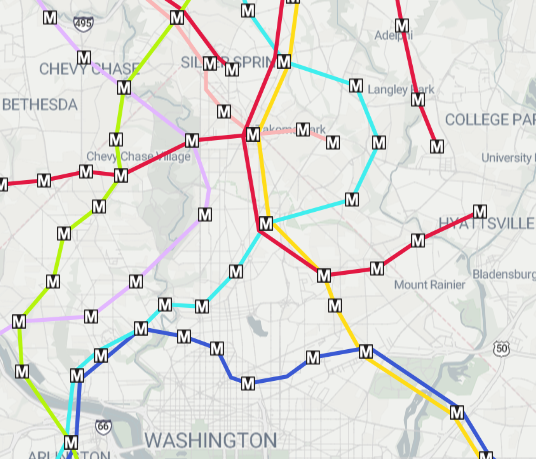
\includegraphics[width=0.3\textwidth]{./img/aco.png}
    \caption{Transit network generated by the ACO algorithm.}
    \label{fig:aco_network}
    \Description{A map visualizing the transit network generated by the Ant Colony Optimization algorithm, with lines and stations highlighted.}
\end{figure}

\begin{figure}[ht]
    \centering
    \includegraphics[width=0.3\textwidth]{./img/naive.png}
    \caption{Transit network generated by the naive (random walk) algorithm.}
    \label{fig:naive_network}
    \Description{A map visualizing the transit network generated by the naive (random walk) algorithm, with lines and stations highlighted.}
\end{figure}

\subsection{Evaluation Results}
Table~\ref{tab:eval_basic} reports basic coverage and access metrics for all variants. Table~\ref{tab:eval_equity} summarizes equity and population coverage at multiple walk radii, and Table~\ref{tab:eval_efficiency} reports service efficiency and transfer burden. For context, the real WMATA system is approximately 129 route miles (208 km) with 98 stations~\cite{lit:wmata_wikipedia}. The \textit{track\_km} column below is a service-track measure derived from line-segment lengths (interlined segments counted multiple times) and is therefore not directly comparable to route miles, but it provides a consistent internal length basis across all generated networks and WMATA.

\begin{table*}[h]
\caption{Basic Coverage and Access Metrics. \textit{pop\_in\_catchments} is a relative KDE density mass integrated over station catchments, not an absolute population count; use only for comparing variants.}
\label{tab:eval_basic}
\resizebox{\textwidth}{!}{
\begin{tabular}{lccccc}
\toprule
\textbf{Network} & \textbf{pt\_cov\%} & \textbf{neigh\_cov\%} & \textbf{avg\_dist\_region\_m} & \textbf{avg\_dist\_dc\_m} & \textbf{pop\_in\_catchments} \\
\midrule
Naive & 14.24 & 5.79 & 10038 & 1241 & 0.0184 \\
Iterative & 16.46 & 7.02 & 12518 & 991 & 0.0213 \\
ACO & 11.00 & 3.99 & 8642 & 1697 & 0.0168 \\
Genetic & 13.06 & 5.79 & 10206 & 1219 & 0.0175 \\
WMATA & 10.34 & 3.03 & 15341 & 1630 & 0.0098 \\
\bottomrule
\end{tabular}
}
\end{table*}

\begin{table*}[h]
\caption{Equity and Population Coverage}
\label{tab:eval_equity}
\resizebox{\textwidth}{!}{
\begin{tabular}{lccccc}
\toprule
\textbf{Network} & \textbf{pop\_gini} & \textbf{cov\_250m\%} & \textbf{cov\_500m\%} & \textbf{cov\_1km\%} & \textbf{high\_need\_cov\%} \\
\midrule
Naive & 0.503 & 2.1 & 7.9 & 25.7 & 10.1 \\
Iterative & 0.463 & 2.6 & 9.4 & 29.8 & 12.8 \\
ACO & 0.498 & 2.0 & 7.5 & 24.0 & 8.6 \\
Genetic & 0.501 & 1.8 & 7.4 & 25.3 & 9.3 \\
WMATA & 0.546 & 1.0 & 4.3 & 13.5 & 6.0 \\
\bottomrule
\end{tabular}
}
\end{table*}

\begin{table*}[h]
\caption{Service Efficiency and Transfer Burden}
\label{tab:eval_efficiency}
\resizebox{\textwidth}{!}{
\begin{tabular}{lcccccc}
\toprule
\textbf{Network} & \textbf{track\_km} & \textbf{pop\_per\_km} & \textbf{mean\_xfers} & \textbf{0xfer\%} & \textbf{1xfer\%} & \textbf{2+xfers\%} \\
\midrule
Naive & 1434.5 & 0.26 & 1.04 & 14.0 & 68.5 & 17.5 \\
Iterative & 1425.9 & 0.31 & 0.81 & 20.5 & 77.9 & 1.6 \\
ACO & 1438.6 & 0.25 & 0.87 & 21.7 & 69.9 & 8.4 \\
Genetic & 1383.4 & 0.25 & 0.91 & 19.8 & 69.0 & 11.2 \\
WMATA & 344.1 & 0.59 & \textit{N/A} & \textit{N/A} & \textit{N/A} & \textit{N/A} \\
\bottomrule
\end{tabular}
}
\end{table*}

Several patterns emerge from the evaluation data. The iterative network is the strongest overall performer, leading on point coverage (16.46\%), neighborhood coverage (7.02\%), 1\,km population coverage (29.8\%), high-need coverage (12.8\%), population in catchments (0.0213), and Gini coefficient (0.463)---the most equitable distribution of transit access across stations. The naive network is competitive, ranking second on point coverage (14.24\%) and tying the genetic variant on neighborhood coverage (5.79\%), while posting the second-best DC intra-city average distance (1,241\,m). The ACO and genetic networks perform broadly similarly on coverage and efficiency, with point coverage of 11.0--13.1\% and pop\_per\_km of 0.25 for both.

A notable finding is that the current ACO network's average distance to a station within DC (1,697\,m) now exceeds WMATA's (1,630\,m), meaning the ACO variant provides worse intra-city DC access than the real metro system despite outperforming it regionally. This reflects the single-generation ACO configuration in the current pipeline, which does not allow sufficient pheromone accumulation to concentrate routes on the dense urban core. WMATA still leads all generated variants on service efficiency (pop\_per\_km 0.59), consistent with its purpose-built design for high-ridership corridors. The four generated networks are more similar to one another than in prior evaluations, all clustering between 1,383--1,439\,km of service track and 11.0--16.5\% point coverage. This convergence reflects both the stabilized contracted Gabriel graph and the practical effect of running each algorithm on the same underlying search space.

These results show that algorithmic networks can meaningfully outperform the existing metro on coverage and equity metrics, but real-world feasibility requires balancing those gains against transfer burden and track length. The iterative variant offers the strongest case for a balanced design, combining the widest coverage with the most equitable station distribution and a manageable transfer burden. Given WMATA's real-world system---208\,km, 6 lines, 98 stations~\cite{lit:wmata_wikipedia}---compared to the 20-line generated networks, the coverage advantages must be understood in the context of this scale difference. The generated networks represent aggressive build-out scenarios rather than direct replacements at current capital scale; a fair comparison would require normalizing by number of lines or total route length.

I also perform some potential use-case evaluation by identifying location pairs and calculating the transit time in each network. I calculate the transit times for my network using my Route Planner tool, and I calculate transit times for the real-world network using the WMATA transit planner application. In this report I compare the results obtained for three sample itineraries chosen to demonstrate a variety of transit uses and to address the shortcomings of the existing WMATA network that I raised in the introduction. The three routes presented in this paper are: College Park to DCA Airport (suburb to important hub), downtown Bethesda to Reston Center (suburb to suburb), and Congress Heights to downtown Silver Spring (disadvantaged neighborhood to suburb). For all three routes, the algorithms developed in this project provide faster transit times than the real-world network, with each algorithm having stronger performance on different routes. Travel times for three of the four generated variants are included in Table~\ref{tab:transittimes}. Table \ref{tab:transittimes} shows the travel times calculated for each network. 

% --- Table: Sample Transit Times ---
\begin{table*}[h]
\caption{Sample Transit Times for Selected Origin-Destination Pairs}
\label{tab:transittimes}
\resizebox{\textwidth}{!}{
\begin{tabular}{lccc}
\toprule
\textbf{Network} & \textbf{College Park $\rightarrow$ DCA} & \textbf{Bethesda $\rightarrow$ Reston} & \textbf{Congress Heights $\rightarrow$ Silver Spring} \\
\midrule
Genetic & 29 min & 41 min & 30 min \\
ACO & 1 hr 29 min & 1 hr 10 min & 35 min \\
Iterative & 37 min & 1 hr 1 min & 19 min \\
Naive & 32 min & 32 min & 17 min \\
\midrule
Real-world & 43 min & 1 hr 7 min & 41 min \\
\bottomrule
\end{tabular}
}
\end{table*}

Visual comparison of the generated networks provides additional context. The naive network achieves competitive point and neighborhood coverage relative to the other generated variants, consistent with the principle that 20 constrained random walks produce serviceable coverage through volume rather than directed optimization.

The iterative network is the most balanced performer. Its Gini coefficient (0.463) indicates a relatively uniform distribution of transit access, and it leads on most coverage metrics. Its 0-transfer share (20.5\%) is lower than in some prior evaluations, reflecting reduced opportunities for line alignment overlap in the current contracted graph; fewer station pairs can therefore be served without a transfer.

The ACO network, constrained to a single generation in the current pipeline configuration, produces a more compact and operationally coherent solution than in prior runs: mean transfers have improved to 0.87 and the 2\texttt{+} transfer share has fallen to 8.4\%. However, its spatial coverage has contracted and its average intra-DC station distance (1,697\,m) now lags behind both the real WMATA system and all other generated variants. Running ACO for additional generations would likely recover coverage, as longer pheromone accumulation expands the region of the solution space explored.

The genetic algorithm produces a network of comparable scope to the other generated variants, with the shortest service track (1,383.4\,km) and coverage metrics broadly in line with naive and ACO. The service-pattern reward in the fitness function does not produce an outsized network under the current parameterization, and all efficiency metrics are consistent with the other generated networks.

\subsection{Limitations}
The quality of the networks generated using my pipeline are only as good as the data they are created from. As discussed earlier, the data portals for each of the states varied wildly with respect to data depth and breadth. Virginia, in particular, did not have nearly as much data containing locations of areas supported by transit. Maryland and Washington, D.C. both had much more comprehensive data resources, which is expected given that Washington, D.C. is a single municipal jurisdiction and Maryland is a relatively small state mostly centered around a single metropolitan area. Virginia, on the other hand, is a large state with many metropolitan areas, and the data reflected this. There were often data of the sort I was interested in, but only for one or two counties and outside the DC area. 

The method of combining point data from multiple sources and creating a KDE from multiple sources entailed several limitations: first, each data point was treated as having the same transit importance, and the KDE therefore acted as a map of the amount of points in a given area. This means that the KDE scoring returned high values for regions that were well covered by the existing data, and low values for those with poor coverage, and no weight to whatever relative importance may have existed between points. The overall takeaway is that the transit algorithms produce plausible-looking networks partly because geometric constraints guide routes along natural alignments, and partly because a large number of generated lines provides broad coverage by volume. The data-driven demand scoring shapes the spatial concentration of these lines but cannot substitute for the hard connectivity requirements that real-world transit planning specifies. Across the four algorithms, results are more similar in scale than in prior runs but still often leave densely populated neighborhoods underserved, as evidenced by high-need coverage rates of 8.6--12.8\% across all generated variants. Across algorithms, travel times between destination pairs remain broadly similar, which is likely because with sufficient network density, one- or two-transfer routes on fairly straight alignments are possible between most urban destinations. It is also important to note that my network's reported high performance as compared to the real-world network is also likely largely attributable to the length and number of lines. Each algorithm produces a 20-line network, as compared to the real-world network which has six lines. 

In general, the method I have created in this project does not largely reflect the priorities or procedures of real-world transit agencies. Transit networks are not decided by random algorithms applied across entire metropolitan areas. The search space of the problem is still too great; there were not enough hard constraints on which areas the network should have connected. The result is a network that reaches most necessary areas because the number of randomly-generated lines is high enough. 

\subsection{Implications for Urban Transit Planning}
Despite the many shortcomings of the procedure inherent to this project, it still serves as a valuable tool at encouraging ambition and imagination in public transit planning. Although a 20-line metro system for the Washington metropolitan area would potentially cost hundreds of billions of dollars to construct, it would not be the first transit network of its size in the United States. The networks generated in this project are similar in density and robustness to the New York City Subway, which operates 28 service patterns across over 1000 km of track. New York City is far beyond all other American cities at reducing car usage, which is largely attributable to the coverage, speed, and dependability of its subway network. Although the New York metropolitan area is nearly three times as large as the Washington metropolitan area, the New York Subway does not expand beyond city limits into the suburbs, and the population within New York city limits of around 9 million is much more comparable to the population of the Washington metropolitan area. Therefore, a rapid transit network for the Washington metropolitan area that is significantly larger than the existing network would not be without comparison. 

\subsection{Future Work}

I hope to apply the general procedure of this work to create similar transit maps for other metropolitan areas in the United States. Graph neural network node scoring and an Ant Colony Optimisation metaheuristic have now been implemented; future work could explore training a graph-level generative model that produces complete route sets end-to-end rather than scoring individual nodes, as well as integrating real fare-elasticity data into the ridership model to improve boarding estimates. More granular ROW classification---distinguishing, for example, between new tunnels and conversion of existing underground freight corridors---would improve cost accuracy. Incorporating population growth projections and LODES employment forecasts would allow evaluation of network designs under future demand scenarios. 

\section{Acknowledgments}

I thank my instructors and peers at the University of Maryland for their feedback and support. I also acknowledge the open data providers, including the US Census Bureau, city- and state-level open data providers, and transit providers.

\bibliographystyle{ACM-Reference-Format}
\bibliography{sample-base}

\end{document}
